\documentclass{../source/Experiment}

\major{信息工程}
\name{姚桂涛}
\title{波导传输线负载特性测量与阻抗匹配}
\stuid{3190105597}
\college{信息与电子工程学院}
\date{\today}
\lab{东4-221}
\course{电磁场与电磁波}
\instructor{王子立}
\grades{}
\expname{波导传输线负载特性测量与阻抗匹配}
\exptype{}
\partner{华天择}

\usepackage{caption}

\DeclareCaptionLabelSeparator{twospace}{\, }
\captionsetup{labelsep = twospace}

\begin{document}
    \makecover
    \makeheader

    \section{实验目的}
    了解波导传输线的基本特性,容性膜片的负载特性及阻抗匹配方法。
    
    覆盖的基本概念:
    \begin{itemize}
        \item 波导的传输线模型
        \item 波导色散特性——波导波长
        \item 阻抗及匹配
        \item Smith圆图
    \end{itemize}

    \section{实验过程及结果}

        \subsection{工作频率$ƒ$测量}
            \begin{enumerate}
                \item 测量线开口端用短路块短接。
                \item 接通固态微波信号源,工作状态选择方波调制。
                \item 调节波导检波器中的短路活塞或三销钉调配器使示波器上显示的检波输出(方波)幅度最大。如果示波器上显示的输出幅度还不够大,可适当减少可调衰减器的衰减量,反之增加可调衰减器的衰减量。(注意:由于微波频率高,波长短,故调节时必须如同调节显微镜一样细心,而且在用三销钉调节时,销钉插入深度不能超过波导高度$b $的一半,否则会产生全反射以至无信号检出。)
                \item 用直读式频率计测量此时系统的工作频率$ƒ$(注意:调节时必须缓慢细调,由于频率计等效于电路中的一个并联谐振回路,当它产生谐振时,一部份能量被吸收,相应地串接在后面的检波器得到的能量就变小,于是示波器上看 到的方波幅度也就变小,因而调节时注意观察示波器上的方波幅度, 当看到幅度有突变,且变得最小时,频率计上读得的读数就是微波信号源的振荡频率,单位为$GHz$。频率计的读法是:两条水平红线夹着的那一行刻度线与垂直红线相交的那一点的刻度数值),记录到实验记录本上。
            \end{enumerate}

            实验数据:$$f = 9.51GHz$$

            \begin{figure}[H]
                \centering
                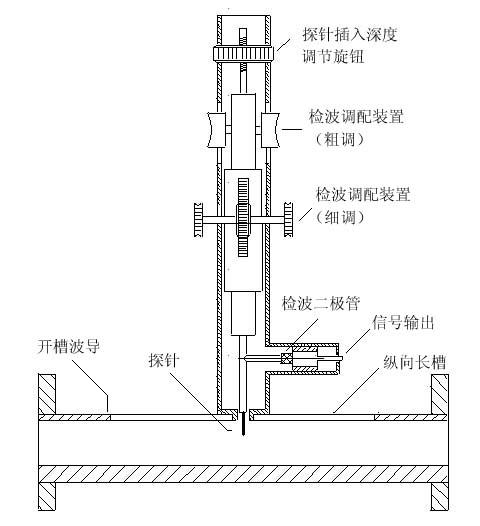
\includegraphics[width = 0.4\textwidth]{pic/波导驻波测量线结构示意}
                \caption{波导驻波测量线结构示意}
            \end{figure}

        \subsection{波导波长测量}
            \begin{enumerate}
                \item 先调节测量线探针插入深度为$1mm $左右,再细心调节测量线上的检波调配装置,使数字万用表上指示的检波输出信号最大,即检波匹配(注意:为使测量线的检波二极管工作在小信号的平方率检波区,探针插入深度不能太深,否则探针本身会引起较大反射,使测量数值产生较大误差)。沿波导横向移动驻波测量探针,使探针位于驻波波腹点(检波的输出最大),此时再调节衰减器使数字万用表读数为$0.500mV$(设定信号在合适的大小),记录此时衰减器的刻度,以便之后测量。
                \item 慢慢地横向移动测量线探针,记下相邻两个驻波波节点的位置$d_{min1}$、$d_{min2}$的刻度值。
            \end{enumerate}
            实验数据:$$d_{min1} = 63.5mm, \qquad d_{min2} =41.8mm \qquad$$

        \subsection{容性膜片等效负载的测量}
        实验装置仍如图2。实验步骤如下:
            \begin{enumerate}
                \item 测量线开口端接短路块,横向移动测量线探针,找到一个驻波波节点位置$d_{min1(\mbox{短})}$并作记录(即等效短路面位置)。
                \item 拆下短路块,接上容性膜片+匹配负载,从$d_{min1(\mbox{短})}$位置往振荡源信号方向移动驻波测量线探针位置,测得第一个驻波最小点位置$d_{min1(\mbox{膜片})}$,并作记录。
                
                实验数据:

                $$d_{min1(\mbox{短})} = 41.8mm \qquad d_{min1(\mbox{膜片})} = 37.65\qquad$$
                $$P_{min} = 0.579mV\qquad P_{max} = 2.233mV\qquad$$

                \item 测量此时的驻波系数,即横向移动驻波测量线探针位置,在数字万用表上读出检波输出最大值$P_{max}$与最小值 $P_{min}$ (注意:考虑到检波器为小信号平方率检波,故数字万用表读出的数值应为相对功率值)。
            \end{enumerate}

            \begin{figure}[H]
                \centering
                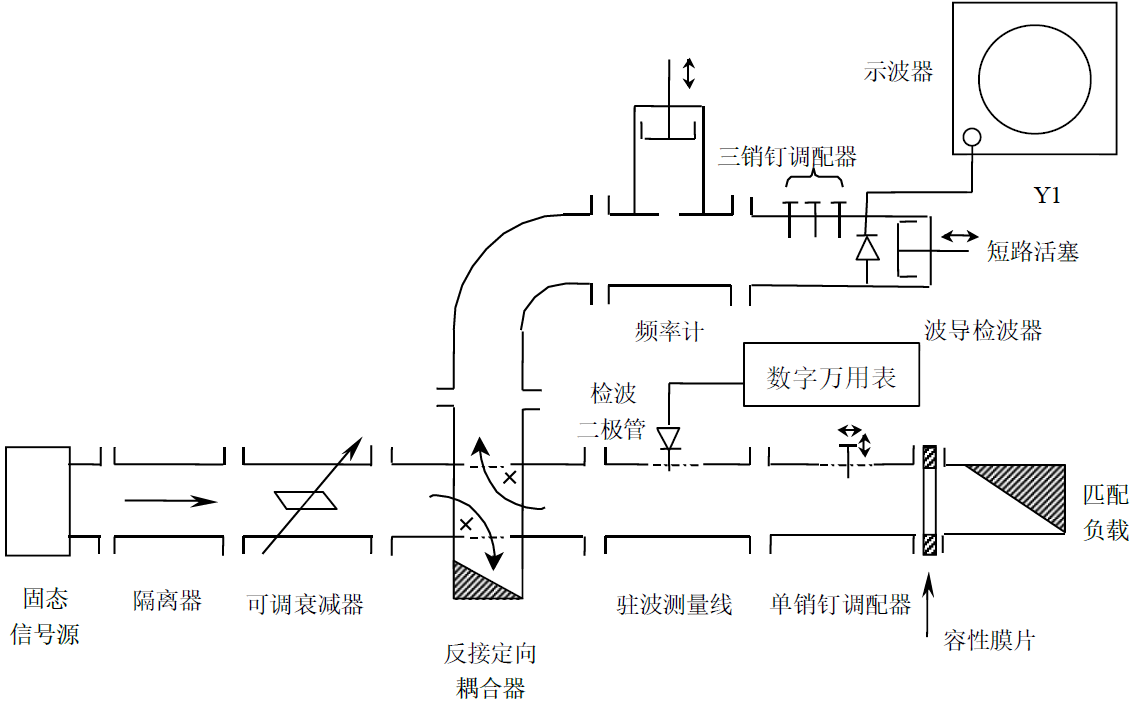
\includegraphics[width = 0.9\textwidth]{pic/1-4.png}
                \caption{}
            \end{figure}

        \subsection{阻抗匹配测量}
        在测量线与容性膜片+匹配负载之间串接一只单销钉调配器。见图2。单销钉调配器是一个其销钉插入波导深度和纵向位置都可以调节的器件。
        \begin{enumerate}
            \item 调节衰减器衰减量,使示波器有足够的方波信号显示。
            \item 细心调节销钉调配器销钉的横向位置和插入波导的深度,使示波器上显示的信号最小(最好能到零)。进而提高示波器的灵敏度和增加输入功率,重复上一调节过程直到当示波器的灵敏度为最高和输入功率为最大且又在示波器上观察到的信号为最小为止,即找到最佳匹配位置。
            \item 适当增加可调衰减器的衰减量之后,横向移动驻波测量线,记录该输入功率下数字万用表上的$P_{max(\mbox{匹配})}$与 $P_{min(\mbox{匹配})}$,并计算此时的驻波系数 。
        \end{enumerate}
        实验数据:$$P_{max(\mbox{匹配})} = 4.218mV\qquad P_{min(\mbox{匹配})} = 1.379mV\qquad$$


    \section{实验结果分析}
        \subsection{计算波导波长$\lambda$}

        $\lambda_g = 2\times |d_{min1}-d_{min2}| = 4.340cm$

        \subsection{计算$TE_{10}$模的波导波长$\lambda_g$,并比较}


        $\lambda = \displaystyle \frac{c}{f} = 3.156cm$

        $\lambda_{g}= \displaystyle \frac{\lambda}{\sqrt{1-\left(\frac{\lambda}{2 a}\right)^{2}}} = 4.358cm$


        计算误差为:$0.87\% $

        \subsection{计算$\rho $,读出$\Gamma $和归一化阻抗值。}

        $\rho = \sqrt{\displaystyle \frac{P_{max}}{P_{min}}} = 1.964$

        计算反射系数:

        $\Gamma = \displaystyle \frac{\rho-1}{\rho+1} = 0.325$

        计算出归一化阻抗为:


        \subsection{计算用单销钉调节匹配后的驻波系数。}
        $P_{max(\mbox{匹配})} = 4.218mV\qquad P_{min(\mbox{匹配})} = 1.379mV\qquad$

        $\rho = \sqrt{\displaystyle \frac{P_{max}}{P_{min}}} = 1.75$

        \subsection{计算匹配状态时销钉所呈现的归一化电抗值。}
        


        \subsection{回答问题:}
            \begin{enumerate}
                \item 测量线开口端不接短路块,任意接一负载,能否测出波导波长?接短路块测波导波长有什么优点?
                不一定。如果接入的负载匹配,则无法测出。\par 
            接短路块时,波节点电压为0,能保证可以通过测相邻波节点到该点的距离测得波长。
                \item 测负载驻波相位为什么要先测$d_{min}$?
                
                为了得到一个参照点,此参照点可以作为短路点的等效位置,从而减小测量误差。
                \item 在单销钉调配器调配前,测量线探针为什么不能伸入到波导里面?
                
                如果探针伸入太多,则探针本身会产生反射,从而造成实验误差。探针伸入超过1/2个矩形波导宽度时,会发生全反射,使实验无法正常进行。
                \item 为什么检波器输出指示越小,表示调配得越好?
                
                检波器测量的是交变的小信号。指示值越小,表示幅值变化的分量占比小。
                \item 如果经销钉调配器调配后,测得驻波系数为1 ,在单销钉调配器与负载之间是否是行波?单销钉调配器至信号源方向是否是行波?为什么?

                单销钉匹配器和负载之间:不是行波
                
                因为这段的传输线没有经过匹配,电压波腹点是电流波节点,这种分布为驻波。
    
                单销钉匹配器至信号源之间:行波
                
                驻波系数为1时,电压电流沿传输线没有变化,为行波。
                

            \end{enumerate}
    \section{实验总结与心得体会}
        本次实验过程操作过程虽然比较简单,可以直接根据实验的教程很快做出来。但是本次实验却并不简单。主要问题在于难以将理论课学习的知识和实验相联系起来。经过本次实验,我对于理论课学习到的知识有了更加深刻的理解。
\end{document}